\documentclass[conference]{IEEEtran}
\IEEEoverridecommandlockouts
\usepackage{cite}
\usepackage{amsmath,amssymb,amsfonts}
\usepackage{algorithmic}
\usepackage{graphicx}
\usepackage{textcomp}
\usepackage{xcolor}
\usepackage{lipsum}
\usepackage{blindtext}
\usepackage{subfig}
\usepackage{caption}
\usepackage{placeins}
\usepackage{afterpage}
\graphicspath{{./images/}}

\def\BibTeX{{\rm B\kern-.05em{\sc i\kern-.025em b}\kern-.08em
    T\kern-.1667em\lower.7ex\hbox{E}\kern-.125emX}}

\begin{document}

\title{Deep Reinforcement Learning with the MuJoCo Physics Simulator}

\author{
    \IEEEauthorblockN{Curtis Brinker}
    \IEEEauthorblockA{cjbzfd@mst.edu}
    \and
    \IEEEauthorblockN{Tanner May}
    \IEEEauthorblockA{tmay@mst.edu}
}
\maketitle

\begin{abstract}
    \blindtext
\end{abstract}

\section{Introduction}

Recent developments in machine learning have made huge strides in approaching problems that were previously unsolvable with traditional programming methods.
In general, machine learning techniques are grouped into three categories: supervised learning, unsupervised learning, and reinforcement learning. \cite{rl_application}

\blindtext
\blinditemize[4]

\blindtext

\section{Testing Environment}

\blindtext
\blinditemize[4]

\blindtext

\section{Background}

\blindtext

\subsection{Advantage Actor Critic (A2C)}

\blindtext

\subsection{Deep Deterministic Policy Gradient (DDPG)}

\blindtext

\subsection{Soft Actor Critic (SAC)}

\blindtext

\section{Methodology}

\blindtext

\section{Results}

\blindtext

\subsection{CartPole-v0}

\blindtext

\subsection{Pendulum-v1}

\begin{figure}
    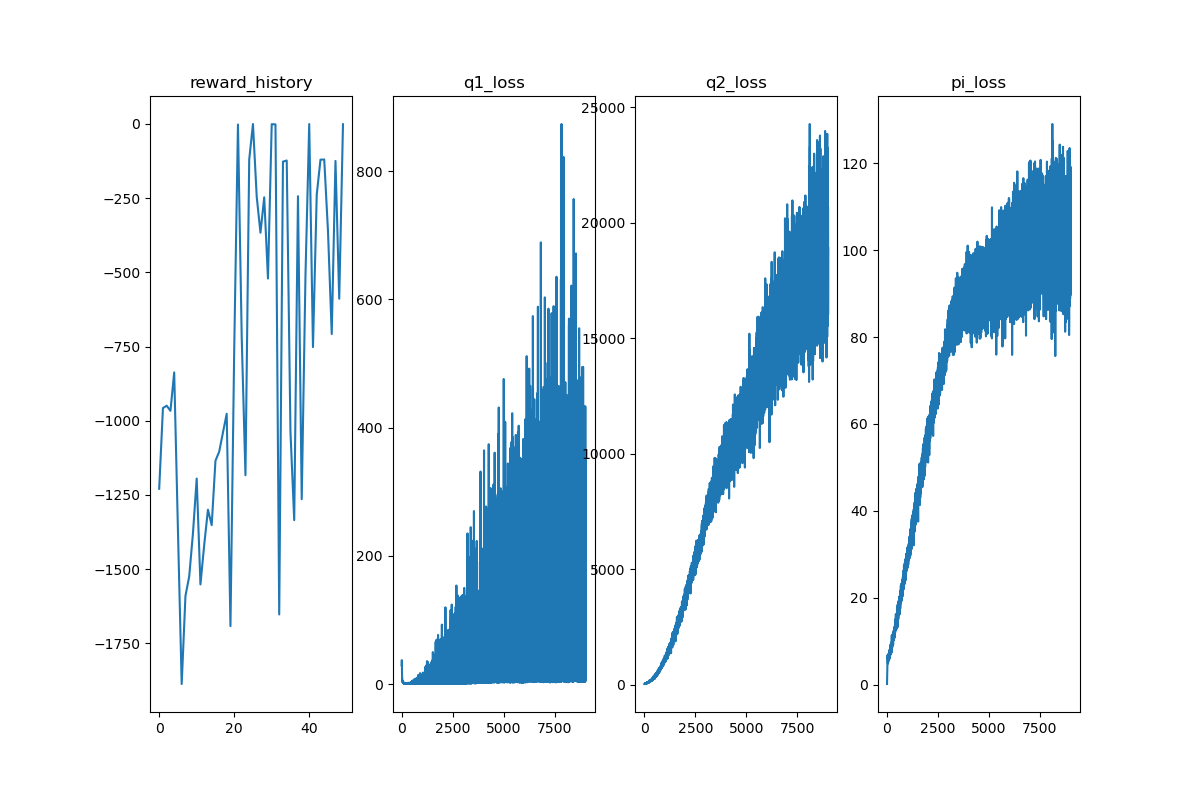
\includegraphics[width=0.45\textwidth]{sac-pendulum}
    \caption{SAC in the Pendulum-v1 Environment}
\end{figure}

\blindtext

\subsection{Ant-v3}

\begin{figure}
    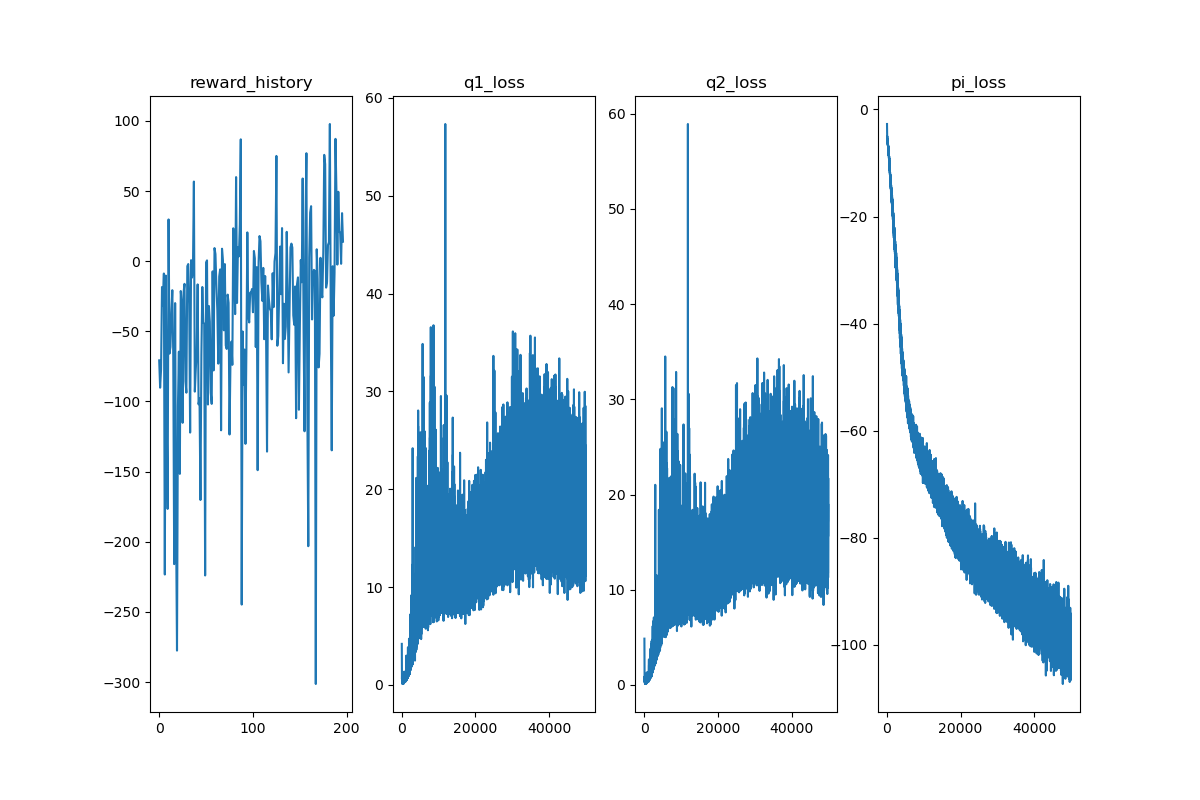
\includegraphics[width=0.45\textwidth, height=5cm]{sac-ant}
    \caption{SAC in the Ant-v3 environment}
\end{figure}

\begin{figure}
    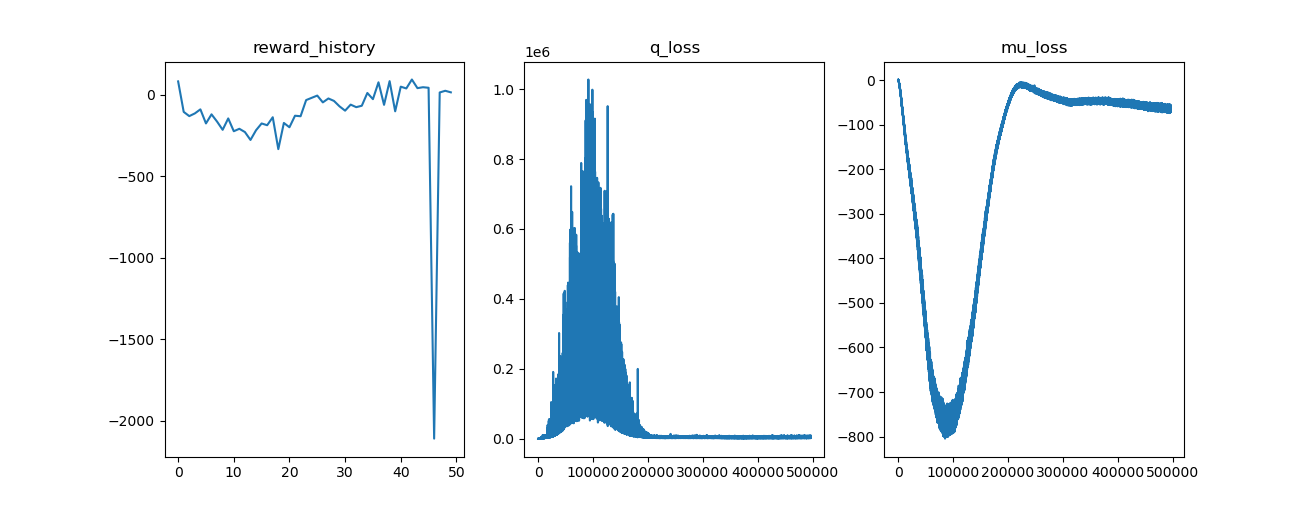
\includegraphics[width=0.45\textwidth, height=5cm]{ddpg-ant}
    \caption{DDPG in the Ant-v3 environment}
\end{figure}

\blindtext

\subsection{Humanoid-v3}

\blindtext

\section{Future Work and Conclusions}

\blindtext[2]


\bibliography{references}
\bibliographystyle{ieeetran}


\end{document}
